\subsection{Example \#2: dependence model between two time-series}
\label{S:ExampleDispTemp}

\subsubsection{Data description}

This example uses two synthetic time series that mimics displacement and temperature data measured on a bridge.
The  Figure~\ref{fig:DataSummaryRaw2}a shows that data points exist between August 2013 and October 2015.
The timestep is non-uniform; it varies from 1 hour to 25 hours (see Figure~\ref{fig:DataSummaryRaw2}b). 
The timestep vector is not identical on each time series. 
It means that the time-series are not synchronized between each other.
The most frequent (i.e referent) time step is 1 hour for both time-series (Section~\ref{SS:NonUniform}).
There is no missing data (NaN) on the displacement time-series, but there are missing data on the temperature time series as indicated by the red crosses on the Figure~\ref{fig:DataSummaryRaw2}c.
Each red cross indicates the presence of a Not a Number (NaN) value in the time series.
After data synchronization, the time step vectors are identical on each time series (Figure~\ref{fig:DataSummaryDefaultPreProcessed2}).
Both time-series are stationary, and they exhibit a level, a yearly and daily periodic pattern as well as an autoregressive pattern.
The periodic patterns observed on the displacement time-series is due to the temperature variations observed in the temperature time series.

\begin{figure*}[h!]
\centering
\begin{subfigure}{\linewidth}
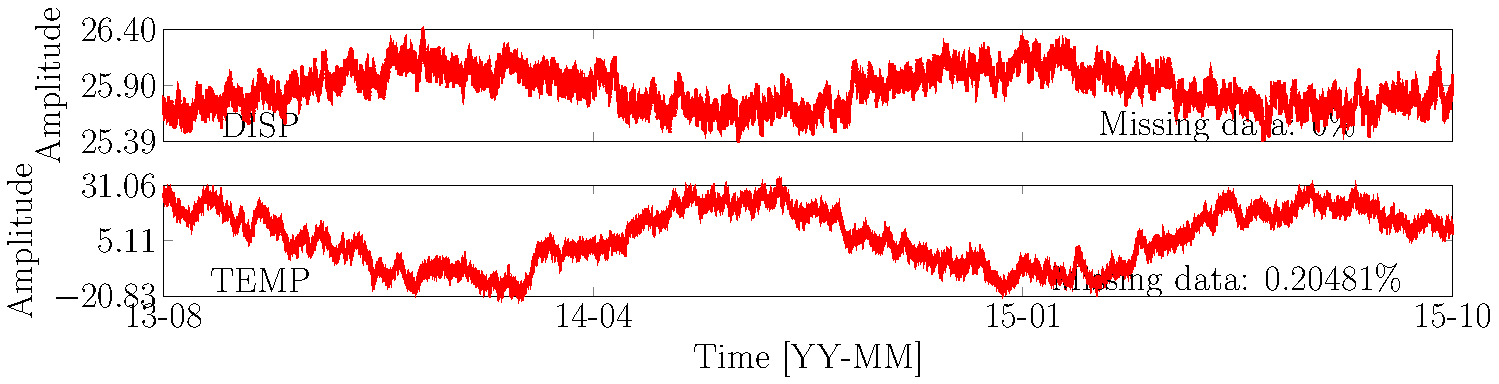
\includegraphics[width=0.9\linewidth]{./docfigs/Example_DISPTEMPSIM/raw/ALL_AMPLITUDES.pdf} 
\caption{Amplitude}
\end{subfigure}
\begin{subfigure}{\linewidth}
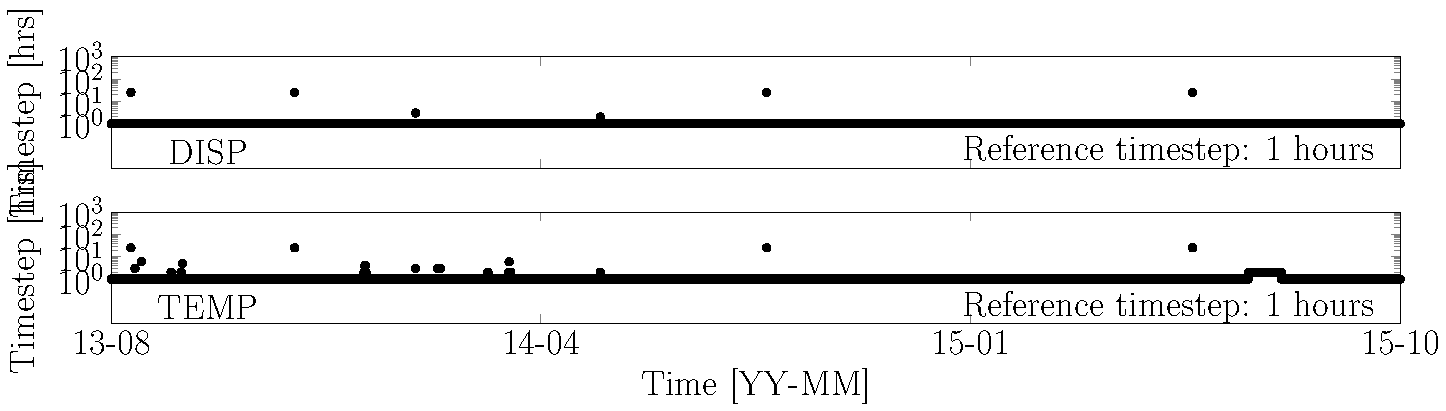
\includegraphics[width=0.9\linewidth]{./docfigs/Example_DISPTEMPSIM/raw/ALL_TIMESTEPS.pdf}
\caption{Timestep}
\end{subfigure}
\begin{subfigure}{\linewidth}
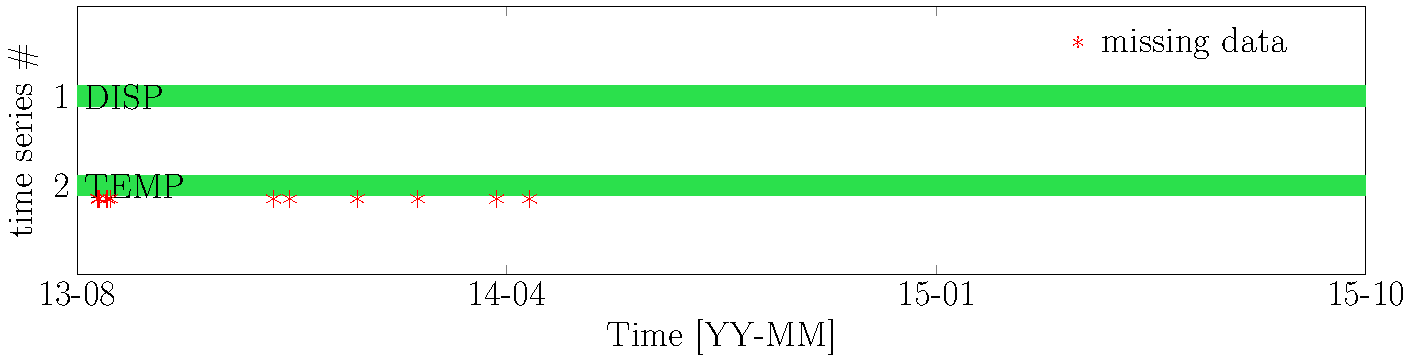
\includegraphics[width=0.9\linewidth]{./docfigs/Example_DISPTEMPSIM/raw/AVAILABILITY.pdf}
\caption{Availability}
\end{subfigure}
\caption{Data used in example \#2.}
\label{fig:DataSummaryRaw2}
\end{figure*}


\begin{figure*}[h!]
\centering
\begin{subfigure}{\linewidth}
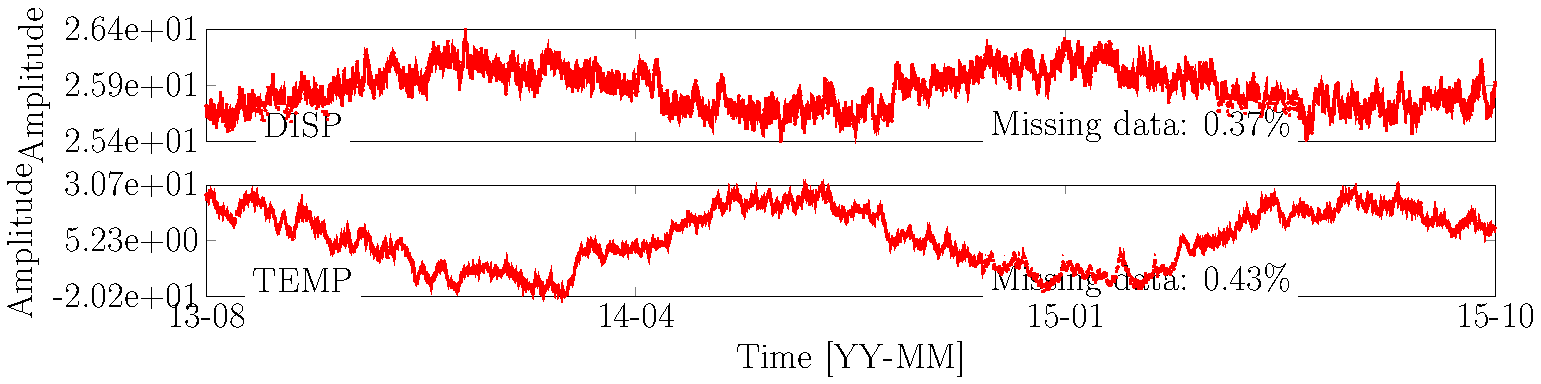
\includegraphics[width=0.9\linewidth]{./docfigs/Example_DISPTEMPSIM/preprocessed_default/ALL_AMPLITUDES.pdf} 
\caption{Amplitude}
\end{subfigure}
\begin{subfigure}{\linewidth}
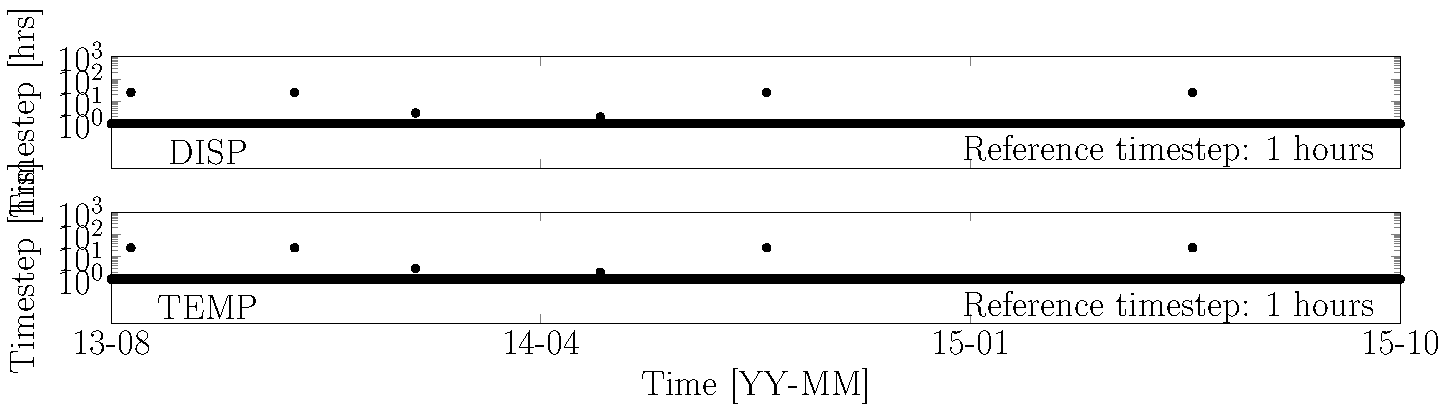
\includegraphics[width=0.9\linewidth]{./docfigs/Example_DISPTEMPSIM/preprocessed_default/ALL_TIMESTEPS.pdf}
\caption{Timestep}
\end{subfigure}
\begin{subfigure}{\linewidth}
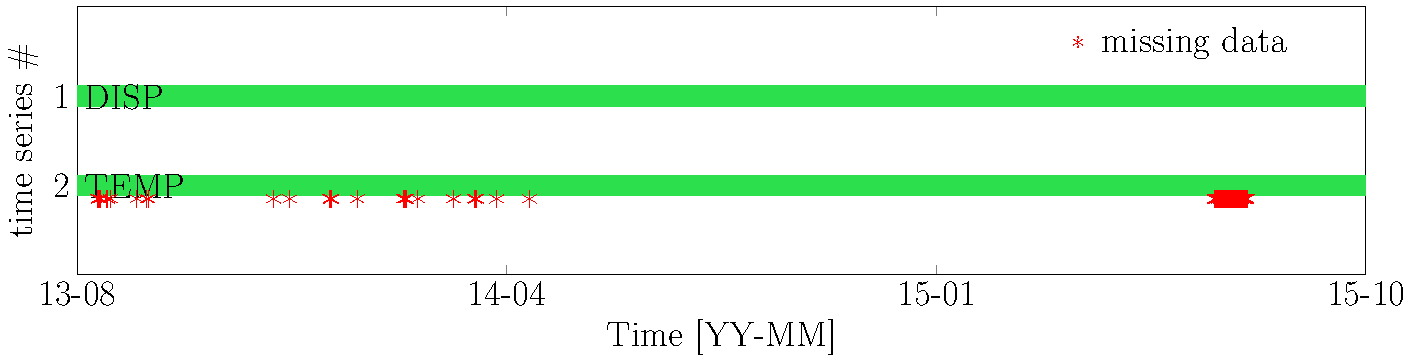
\includegraphics[width=0.9\linewidth]{./docfigs/Example_DISPTEMPSIM/preprocessed_default/AVAILABILITY.pdf}
\caption{Availability}
\end{subfigure}
\caption{Data used in example \#2 after pre-processing.}
\label{fig:DataSummaryDefaultPreProcessed2}
\end{figure*}



\subsubsection{Model description}
\label{SS:ModelConstructionExample2}

The model includes one model class, and the block components are 
\begin{gather*}
\textbf{x}=[x^{\mathtt{LL}}_{\text{D}}, x^{\mathtt{AR}}_{\text{D}}, x^{\mathtt{LL}}_{\text{T}}, x^{\mathtt{P1}\text{,yearly}}_{\text{T}}, x^{\mathtt{P2}\text{,yearly}}_{\text{T}}, x^{\mathtt{P1}\text{,daily}}_{\text{T}} , x^{\mathtt{P2}\text{,daily}}_{T}, x^{\mathtt{AR}}_{\text{T}}].
\end{gather*}
where $\text{D}$ and $\text{T}$ stand for displacement and temperature time-series, respectively.
The periodic patterns observed on the displacement are considered through a dependency of the displacement on the periodic block components of the temperature time-series (Section~\ref{S:Dependencies}).
The associated model parameters are
\begin{align*}
\bm\theta & =[\sigma_{w, \text{D}}^{\mathtt{LL}}, \phi^{\mathtt{AR}}_{D}, \sigma_{w, \text{D}}^{\mathtt{AR}}, \sigma_{v, \text{D}},  \\
&  \sigma_{w, \text{T}}^{\mathtt{LL}},  p^{\mathtt{P}, \text{yearly}}_{\text{T}}, \sigma_{w, \text{T}}^{\mathtt{P}, \text{yearly}} , p^{\mathtt{P}, \text{daily}}_{\text{T}} , \sigma_{w, \text{T}}^{\mathtt{P}, \text{daily}}, \phi^{\mathtt{AR}}_{\text{T}}, \sigma_{w, \text{T}}^{\mathtt{AR}}, \sigma_{v, \text{T}}].
\end{align*}
The optimized model parameters values computed using the Newton-Raphson algorithm (see~\ref{SS:THModelParameterEstimation}) are
\begin{align*}
 \bm\theta^{\text{*}}& =[0, 0.97, 0.019, 7.42\times10^{-7},  \\
 & 0, 365.2422, 0, 1, 0, 0.99, 0.43, 2.67\times10^{-5}, -0.011, 0.0711, 0.000292 ]
\end{align*}
The optimized initial hidden states mean and covariance values are 
\begin{align*}
\bm \mu^{*}_{0} & = [	 25.9  ,	-0.0595	, 5.45  	, 17.6  ,	-0.934	, 0.678 ,	0.41  ,	2.1]^{\intercal}, \text{and} \\
\bm\Sigma^{*}_{0} & = \text{diag} [	3.71\times10^{-5},	0.000457	, 0.287 	, 0.263 ,	0.265 	,8.14\times10^{-5}	, \\
 & 8.14\times10^{-5}	, 0.71    ], 
 \end{align*}
 respectively.
The hidden states computed using the estimated model parameters and initial hidden states are presented in Figure~\ref{fig:DISPTEMPSIMOptimizedOptimizedExample2}.


\subsubsection{Run the example from pre-existing configuration file}
\label{SS:LoadConfigFileEx2}
There is a configuration file CFG\_Example\_DISPTEMP\_optim.m which is located in the ``config\_files'' folder of the OpenBDLM package.
CFG\_Example\_DISPTEMP\_optim.m contains the optimized model parameters and optimized initial hidden states values.
There is also a data file DATA\_Example\_DISPTEMP\_optim.mat that is located in the ``data/mat'' subfolder.
Therefore, it is possible to run the example \#1 by following the following steps from the \MATLAB{} command line:
\begin{enumerate}
\item Start OpenBDLM. Type \colorbox{light-gray}{\lstinline[basicstyle = \mlttfamily \small, backgroundcolor = \color{light-gray}]!OpenBDLM_main('CFG_Example_DISPTEMP_optim.m');!}.
\item Access hidden states estimation menu. Type \colorbox{light-gray}{\lstinline[basicstyle = \mlttfamily \small, backgroundcolor = \color{light-gray}]!3!}.
\item Run the Kalman filter to estimate the hidden states. Type \colorbox{light-gray}{\lstinline[basicstyle = \mlttfamily \small, backgroundcolor = \color{light-gray}]!1!}.
\item Save and quit. Type \colorbox{light-gray}{\lstinline[basicstyle = \mlttfamily \small, backgroundcolor = \color{light-gray}]!Q!}.
\end{enumerate}


\subsubsection{Run the example from command line interaction}

The analysis of a new dataset usually requires to start from scratch.
This section explains how to run the example \#1 from scratch, that is, how to load the data presented in Figure~\ref{fig:DataSummaryRaw2}, configure the model, estimate the model parameters and estimate the hidden states.
This may be done by following the following steps from the \MATLAB{} command line:
\begin{enumerate}
\item Start OpenBDLM. Type \colorbox{light-gray}{\lstinline[basicstyle = \mlttfamily \small, backgroundcolor = \color{light-gray}]!OpenBDLM_main;!}.
\item Choose the interactive tool. Type \colorbox{light-gray}{\lstinline[basicstyle = \mlttfamily \small, backgroundcolor = \color{light-gray}]!0!}.
\item Enter the project name. Type \colorbox{light-gray}{\lstinline[basicstyle = \mlttfamily \small, backgroundcolor = \color{light-gray}]!Example_DISPTEMP!}. 
\item Disregard generating synthetic data. Type \colorbox{light-gray}{\lstinline[basicstyle = \mlttfamily \small, backgroundcolor = \color{light-gray}]!no!}. 
\item Load new data. Type \colorbox{light-gray}{\lstinline[basicstyle = \mlttfamily \small, backgroundcolor = \color{light-gray}]!0!}.
\item Select from the graphical user interface the data files located in the ``/data/csv/Example\_DISPTEMP/'' folder. The Figure~\ref{fig:DataSummaryRaw2} that represents the raw data should popup on screen.
\item Save and continue to perform default pre-processing . Type \colorbox{light-gray}{\lstinline[basicstyle = \mlttfamily \small, backgroundcolor = \color{light-gray}]!7!}. The Figure~\ref{fig:DataSummaryDefaultPreProcessed2} that represents the processed data should popup on screen.
\item Select dependency for the time series \#1. Type \colorbox{light-gray}{\lstinline[basicstyle = \mlttfamily \small, backgroundcolor = \color{light-gray}]![2]!}.
\item Select dependency for the time series \#2. Type \colorbox{light-gray}{\lstinline[basicstyle = \mlttfamily \small, backgroundcolor = \color{light-gray}]![0]!}.
\item Select the number of model classes. Type \colorbox{light-gray}{\lstinline[basicstyle = \mlttfamily \small, backgroundcolor = \color{light-gray}]!1!}. 
\item Select the model block components for time series \#1. Type \colorbox{light-gray}{\lstinline[basicstyle = \mlttfamily \small, backgroundcolor = \color{light-gray}]![11 41]!}.
\item Select the model block components for time series \#2. Type \colorbox{light-gray}{\lstinline[basicstyle = \mlttfamily \small, backgroundcolor = \color{light-gray}]![11 31 31 41]!}.
\item Access hidden states estimation menu. Type \colorbox{light-gray}{\lstinline[basicstyle = \mlttfamily \small, backgroundcolor = \color{light-gray}]!3!}. 
\item Change the state estimation method to UD\footnote{The UD computation is required in this case because of the presence of missing data. See Section~\ref{SS:KFUD} for more details.}. Type \colorbox{light-gray}{\lstinline[basicstyle = \mlttfamily \small, backgroundcolor = \color{light-gray}]!3!}. 
\item Return to the main menu. Type \colorbox{light-gray}{\lstinline[basicstyle = \mlttfamily \small, backgroundcolor = \color{light-gray}]!R!}.
\item Access model parameter estimation menu. Type \colorbox{light-gray}{\lstinline[basicstyle = \mlttfamily \small, backgroundcolor = \color{light-gray}]!1!}. 
\item Start the Newton-Raphson algorithm. Type \colorbox{light-gray}{\lstinline[basicstyle = \mlttfamily \small, backgroundcolor = \color{light-gray}]!1!}. Once the algorithm is converged, the optimized model parameters values should be close to the values presented in Section~\ref{SS:ModelConstructionExample2}. Note also that it is possible to get slightly different values of parameters with the same performance\footnote{Keep in mind that the optimization may take several minutes to several hours. It is possible to abort the analysis here and to load the configuration file called CFG\_Example\_DISPTEMP\_optim.m to load pre-computed values of model parameters, as presented in Section~\ref{SS:LoadConfigFileEx2}.}.
\item Estimate the initial hidden states values. Type \colorbox{light-gray}{\lstinline[basicstyle = \mlttfamily \small, backgroundcolor = \color{light-gray}]!2!}.
\item Estimate the filtered hidden states. Type \colorbox{light-gray}{\lstinline[basicstyle = \mlttfamily \small, backgroundcolor = \color{light-gray}]!1!}. The estimation should be similar to the results presented in Figure~\ref{fig:DISPTEMPSIMOptimizedOptimizedExample2}.
\item Access export menu. Type \colorbox{light-gray}{\lstinline[basicstyle = \mlttfamily \small, backgroundcolor = \color{light-gray}]!17!}. 
\item Export the current project in a configuration file. Type \colorbox{light-gray}{\lstinline[basicstyle = \mlttfamily \small, backgroundcolor = \color{light-gray}]!1!}.
\item Save and quit OpenBDLM. Type \colorbox{light-gray}{\lstinline[basicstyle = \mlttfamily \small, backgroundcolor = \color{light-gray}]!Q!}.
\end{enumerate}




%\subsection{Step 4: configure the model}
%
%The next step is to configure the model.
%First, the program requests the number of model class.
%In this exemple, the time series data looks stationary and we are not interested in anomaly detection, and therefore we type \colorbox{light-gray}{\lstinline[basicstyle = \mlttfamily \small, backgroundcolor = \color{light-gray}]!1!}.
%Secondly, because there are several time series, OpenBDLM needs to know if there are dependencies between the time-series.
%Typing \colorbox{light-gray}{\lstinline[basicstyle = \mlttfamily \small, backgroundcolor = \color{light-gray}]!2!} for the first time-series, and \colorbox{light-gray}{\lstinline[basicstyle = \mlttfamily \small, backgroundcolor = \color{light-gray}]!0!} for the second time series means that the model will consider the irreversible components (if any) of the second (temperature) time-series as covariates to describe the irreversible patterns observed in the first (displacement) time-series.
%Then, OpenBDLM asks for the type of block component for each time-series. 
%Type \colorbox{light-gray}{\lstinline[basicstyle = \mlttfamily \small, backgroundcolor = \color{light-gray}]![11 41]!} for the displacement time series and \colorbox{light-gray}{\lstinline[basicstyle = \mlttfamily \small, backgroundcolor = \color{light-gray}]![11 31 31 41]!} for the temperature time series.
%The yearly and daily periodic patterns observed in the displacement time-series are modelled using the dependence on the periodic components defined for modelling the temperature time series data.
%Note that because an autoregressive component is chosen for the displacement time series data, the time-dependent model error on the displacement is modelled using a dependence on the autoregressive component of the temperature time series data, as well as an independent autoregressive component.
%The  output on \MATLAB{} command window during interactive model configuration is presented in Listing~\ref{LST:OpenBDLMModelConfigureExample2}.
%Type $\dlsh$ to valid.
%The model is then built, a \lstinline[basicstyle = \mlttfamily \small, backgroundcolor = \color{light-gray}]!DATA_DISPTEMP.mat! binary data file, a \lstinline[basicstyle = \mlttfamily \small, backgroundcolor = \color{light-gray}]!CFG_DISPTEMP.m! configuration file, as well as a \lstinline[basicstyle = \mlttfamily \small, backgroundcolor = \color{light-gray}]!PROJ_DISPTEMP.mat! project file are created.
%The OpenBLDM main menu must appear on the \MATLAB{} command window (see Listing~\ref{LST:OpenBDLMMainMenu}).
%Type \colorbox{light-gray}{\lstinline[basicstyle = \mlttfamily \small, backgroundcolor = \color{light-gray}]!Q!} to save and quit.



% \begin{lstlisting}[ frame = single, basicstyle = \mlttfamily \small, caption = { \MATLAB{} command window output during model configuration}, label = LST:OpenBDLMModelConfigureExample2,  float =h!, linewidth=\linewidth, captionpos=b, breaklines=true]
%- Identifies dependence between time series; use [0] to indicate no dependence
%    time serie #1 depends on time series # >> [2]
%
%- Identifies dependence between time series; use [0] to indicate no dependence
%    time serie #2 depends on time series # >> [0]
%
%- How many model classes do you want for each time-series? 
%     choice >> 1
%     
%     ------------------------------------
%          BDLM Component reference numbers
%     ------------------------------------
%     11: Local level 
%     12: Local trend 
%     13: Local acceleration 
%     21: Local level compatible with local trend 
%     22: Local level compatible with local acceleration 
%     23: Local trend compatible with local acceleration 
%     31: Periodic 
%     41: Autoregressive process (AR(1)) 
%     51: Kernel regression 
%     61: Level Intervention 
%     --------------------------------------
%
%- Identify components for time series #1; e.g. [11 31 41]
%     choice >> [11 41]
%
%- Identify components for time series #2; e.g. [11 31 41]
%     choice >> [11 31 31 41]
%
%     Building model...
%     Saving project...
%     Project saved in saved_projects/PROJ_Example_DISPTEMP.mat. 
%     Printing configuration file...
%     Saving data...
%     Database saved in data/mat/DATA_Example_DISPTEMP.mat 
%     Configuration file saved in config_files/CFG_Example_DISPTEMP.m. 
%\end{lstlisting}


%\subsection{Step 5: open the configuration file}
%
%After the data loading and the model configuration, a configuration file named \lstinline[basicstyle = \mlttfamily \small, backgroundcolor = \color{light-gray}]!CFG_Example_DISPTEMP.m! configuration file is automatically created and saved in ``config\_files'' folder.
%Open the configuration file from \MATLAB{} command line by typing  \colorbox{light-gray}{\lstinline[basicstyle = \mlttfamily \small, backgroundcolor = \color{light-gray}]!edit CFG_Example_DISPTEMP.m!}.
%%The first part of this configuration file as it should appear on the \MATLAB{} editor is shown in Listing~\ref{LST:CFGFileExample1}.
%The Model parameters section of the configuration file shows that the model totalizes 15 model parameters, that is 
%\begin{gather*}
%\bm\theta=\{\sigma_{w, \text{D}}^{LL},  \phi^{AR}_{\text{D}}, \sigma_{w,\text{D}}^{AR} ,\sigma_{v,\text{D}},  \\
% \sigma_{w, \text{T}}^{LL}, p^{\text{PD1}}_{\text{T}}, \sigma_{w,\text{T}}^{\text{PD1}} , p^{\text{PD2}}_{T}, \sigma_{w, \text{T}}^{\text{PD2}}, \phi^{AR}_{T}, \sigma_{w, \text{T}}^{AR}, \sigma_{v,\text{T}}, \phi^{\text{D}|\text{T}}_{PD1}, \phi^{\text{D}|\text{T}}_{PD2},  \phi^{\text{D}|\text{T}}_{AR}\}.
%\end{gather*}
%%The default value of the model parameters are assigned  using heuristic knowledge or computed from the data using statistics on the data.
%The default model parameters values are 
%\begin{gather*}
%\bm\theta^{\text{default}}=\{0, 0.75, 0.017, 0.0087, \\
%0, 365.24, 0, 1, 0, 0.75, 1.2905, 0.64526, 0.5, 0.5, 0.5 \}.
%\end{gather*}
%%In the same manner, default value for the initial hidden states are assigned using heuristic knowledge or computed using statistics on the data.
%The default initial hidden states mean  and covariance values are 
%\begin{align*}
% \bm \mu^{\text{default}}_{0} & = [	25.7  ,	0  ,   	16.7  	, 5     ,	0   ,  	5   ,  	0    , 	0        ]^{\intercal}, \text{and} \\
% \text{diag}(\bm\Sigma^{\text{default}}_{0})  & = [	0.122, 	0.0305,	666,   	666,   	666,   	666,   	666 ,  	167     ],
%\end{align*}
%respectively.
%%$\bm \mu^{\text{default}}_{0} = [	25.7  ,	0  ,   	16.7  	, 5     ,	0   ,  	5   ,  	0    , 	0        ]$, and $\text{diag}(\bm\Sigma^{\text{default}}_{0}) = [	0.122, 	0.0305,	666,   	666,   	666,   	666,   	666 ,  	167     ]$, respectively.
%In the Options section, change \lstinline[basicstyle = \mlttfamily \small, backgroundcolor = \color{light-gray}]!misc.options.MethodStateEstimation='kalman'! to \lstinline[basicstyle = \mlttfamily \small, backgroundcolor = \color{light-gray}]!misc.options.MethodStateEstimation='UD'!. 
%In this specific example, the presence of missing data requires the use of UD computations instead of the standard, default, Kalman computation.
%Note that the choice about UD or Kalman is problem dependent. 
%
%\subsection{Step 6: estimate the hidden states}
%
%Type \colorbox{light-gray}{\lstinline[basicstyle = \mlttfamily \small, backgroundcolor = \color{light-gray}]!OpenBDLM_main('CFG_Example_DISPTEMP.m');!} in the \MATLAB{} command line.
%Once, the main menu appears, type  \colorbox{light-gray}{\lstinline[basicstyle = \mlttfamily \small, backgroundcolor = \color{light-gray}]!3!}, then \colorbox{light-gray}{\lstinline[basicstyle = \mlttfamily \small, backgroundcolor = \color{light-gray}]!1!} to estimate the filtered hidden states using the default model parameters and default initial hidden states values.
%The value of the log-likelihood is $-3800091$.
%The estimated hidden states are presented in Figure~\ref{fig:DISPTEMPSIMDefaultDefaultExample2}.


%\subsection{Step 7: estimate the model parameters from the data}
%
%Type \colorbox{light-gray}{\lstinline[basicstyle = \mlttfamily \small, backgroundcolor = \color{light-gray}]!OpenBDLM_main('CFG_Example_DISPTEMP.m');!} in the \MATLAB{} command line.
%Once, the main menu appears, type  \colorbox{light-gray}{\lstinline[basicstyle = \mlttfamily \small, backgroundcolor = \color{light-gray}]!1!}, then \colorbox{light-gray}{\lstinline[basicstyle = \mlttfamily \small, backgroundcolor = \color{light-gray}]!1!} to estimate the model parameters using Newton-Raphson (type  \colorbox{light-gray}{\lstinline[basicstyle = \mlttfamily \small, backgroundcolor = \color{light-gray}]!1!} to use the Stochastic Gradient instead).
%The model parameters learning procedure should start (see for example Listing~\ref{LST:OpenBLDMModelParameterLearning}).
%Note that, by default, OpenBDLM considers that the parameters $\sigma_{w, \text{D}}^{LL}$, $\sigma_{w, \text{T}}^{LL}$, $p^{\text{PD1}}_{\text{T}}$, $\sigma_{w, \text{T}}^{\text{PD1}}$ , $p^{\text{PD2}}_{\text{T}}$, $\sigma_{w,\text{T}}^{\text{PD2}}$ are known.
%Therefore, there are nine model parameters to be learned from the data in this example.
%The estimation of the model parameters may take several hours.
%Therefore, press combinations \colorbox{light-gray}{\lstinline[basicstyle = \mlttfamily \small, backgroundcolor = \color{light-gray}]!Ctrl!} + \colorbox{light-gray}{\lstinline[basicstyle = \mlttfamily \small, backgroundcolor = \color{light-gray}]!c!} to abort the process.
%Once the algorithm is converged, the optimized model parameters values should be close to  \footnote{Note that it is possible to get slightly different value of parameters with the same performance.}
%\begin{gather*}
% \bm\theta^{\text{*}}=\{0, 0.97, 0.019, 7.42\times10^{-7}, 0, 365.2422, 0, 1, 0, 0.99, 0.43, 2.67\times10^{-5},  \\
% -0.011, 0.0711, 0.000292 \}
%\end{gather*}


%\subsection{Step 8: estimate the hidden states using the optimized model parameters. values}
%
%In the ``examples/Example\_DISPTEMP'' folder, there is a configuration file named \lstinline[basicstyle = \mlttfamily \small, backgroundcolor = \color{light-gray}]!CFG_Example_DISPTEMP_optim.m! that contains optimized model parameters estimated using the Newton-Raphson algorithm.
%Copy and paste \lstinline[basicstyle = \mlttfamily \small, backgroundcolor = \color{light-gray}]!CFG_Example_DISPTEMP_optim.m! from  the ``examples/Example\_DISPTEMP'' subfolder  to the ``config\_files'' folder.
%Type \colorbox{light-gray}{\lstinline[basicstyle = \mlttfamily \small, backgroundcolor = \color{light-gray}]!OpenBDLM_main('CFG_Example_DISPTEMP_optim.m');!} in the \MATLAB{} command line to load the configuration file  \lstinline[basicstyle = \mlttfamily \small, backgroundcolor = \color{light-gray}]!CFG_Example_DISPTEMP_optim.m!.
%Once the main menu appears, type  \colorbox{light-gray}{\lstinline[basicstyle = \mlttfamily \small, backgroundcolor = \color{light-gray}]!3!}, then \colorbox{light-gray}{\lstinline[basicstyle = \mlttfamily \small, backgroundcolor = \color{light-gray}]!1!} to estimate the filtered hidden states using the optimized model parameters and default initial hidden states values.
%The value of the log-likelihood is now $38085$.
%The estimated hidden states are presented in Figure~\ref{fig:DISPTEMPSIMOptimizedDefaultExample2}.

%\subsection{Step 9: estimate the initial hidden states}
%
%Type \colorbox{light-gray}{\lstinline[basicstyle = \mlttfamily \small, backgroundcolor = \color{light-gray}]!OpenBDLM_main('CFG_Example_DISPTEMP_optim.m');!} in the \MATLAB{} command line.
%Then, type  \colorbox{light-gray}{\lstinline[basicstyle = \mlttfamily \small, backgroundcolor = \color{light-gray}]!2!}, to optimize the initial hidden states value.
%The estimated initial hidden states mean and covariance values are 
%\begin{align*}
%\bm \mu^{*}_{0} & = [	 25.9  ,	-0.0595	, 5.45  	, 17.6  ,	-0.934	, 0.678 ,	0.41  ,	2.1]^{\intercal}, \text{and} \\
% \text{diag}(\bm\Sigma^{*}_{0}) & = [	3.71\times10^{-5},	0.000457	, 0.287 	, 0.263 ,	0.265 	,8.14\times10^{-5}	, \\
% & 8.14\times10^{-5}	, 0.71    ], 
% \end{align*}
% respectively.
%Once it is done, type  \colorbox{light-gray}{\lstinline[basicstyle = \mlttfamily \small, backgroundcolor = \color{light-gray}]!3!}, and then  \colorbox{light-gray}{\lstinline[basicstyle = \mlttfamily \small, backgroundcolor = \color{light-gray}]!1!} to compute the filtered hidden states using the optimized model parameters and optimized initial hidden states.
%The value of the log-likelihood is $38120$.
%The estimated hidden states are presented in Figure~\ref{fig:DISPTEMPSIMOptimizedOptimizedExample2}.


%\begin{figure*}[h!]
%\centering
%\begin{subfigure}{\linewidth}
%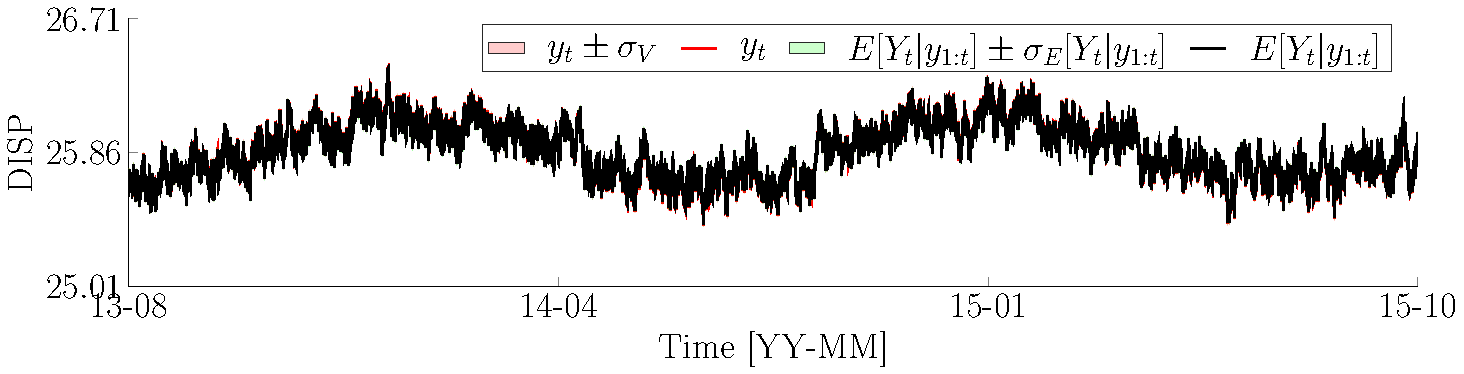
\includegraphics[width=0.9\linewidth]{./docfigs/Example_DISPTEMPSIM/default/DISP_ObservedPredicted.pdf}
%\caption{Observed and estimated displacement data} 
%\end{subfigure}
%\begin{subfigure}{\linewidth}
%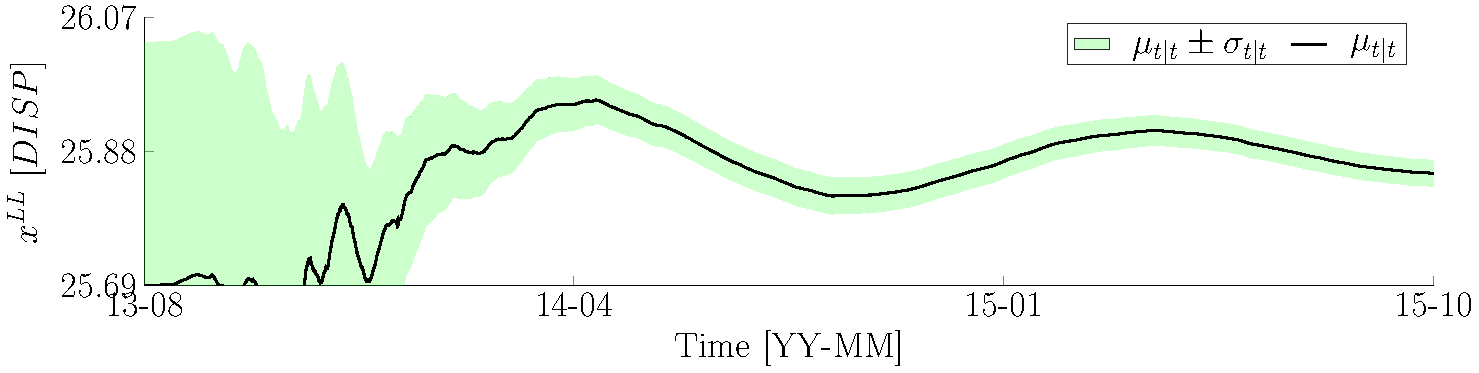
\includegraphics[width=0.9\linewidth]{./docfigs/Example_DISPTEMPSIM/default/DISP_LL_1.pdf}
%\caption{Estimated displacement local level component.}
%\end{subfigure}
%\begin{subfigure}{\linewidth}
%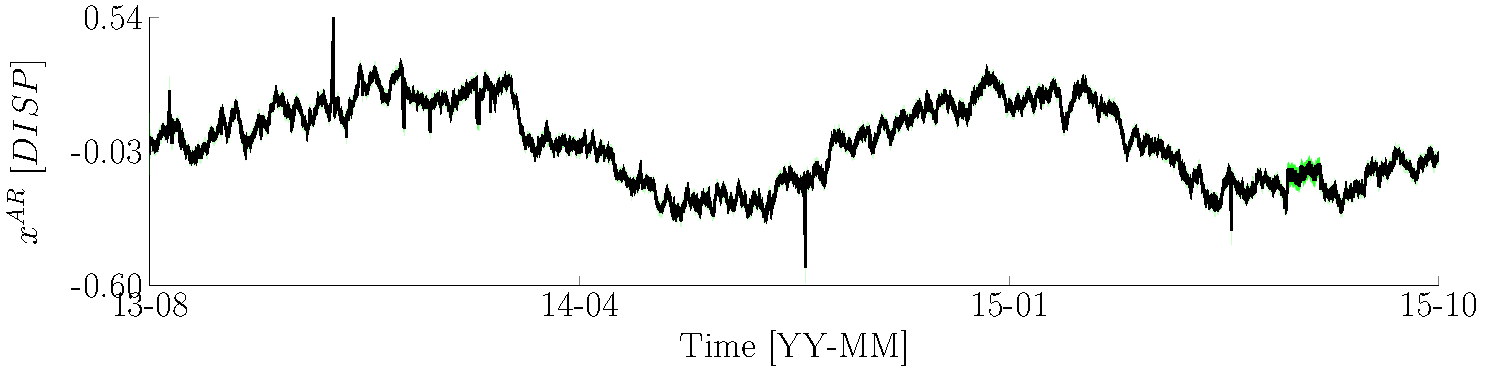
\includegraphics[width=0.9\linewidth]{./docfigs/Example_DISPTEMPSIM/default/DISP_AR_2.pdf}
%\caption{Estimated displacement autoregressive component.}
%\end{subfigure}
%\end{figure*}
%\begin{figure*}[h!]
%\ContinuedFloat
%\begin{subfigure}{\linewidth}
%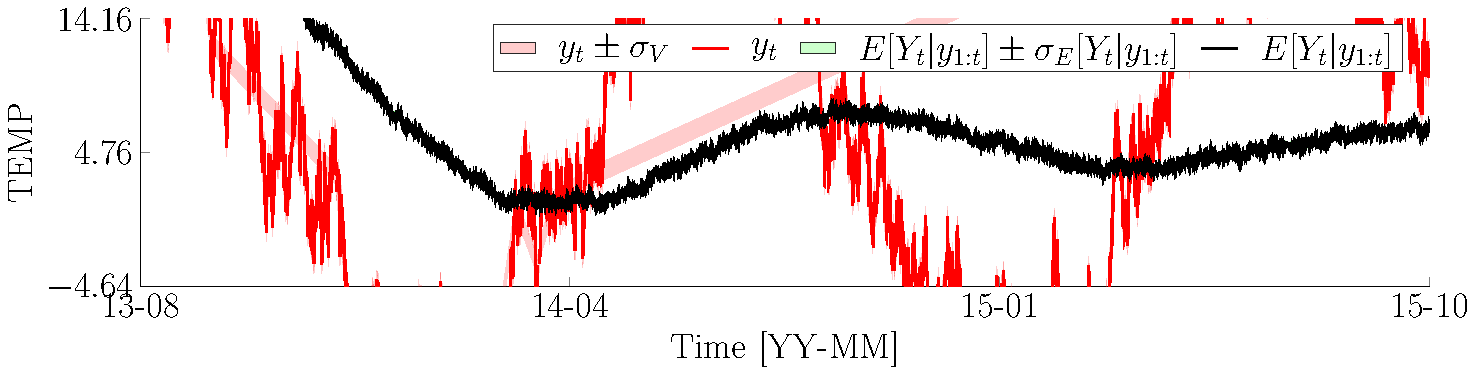
\includegraphics[width=0.9\linewidth]{./docfigs/Example_DISPTEMPSIM/default/TEMP_ObservedPredicted.pdf} 
%\caption{Observed and estimated temperature data}
%\end{subfigure}
%\begin{subfigure}{\linewidth}
%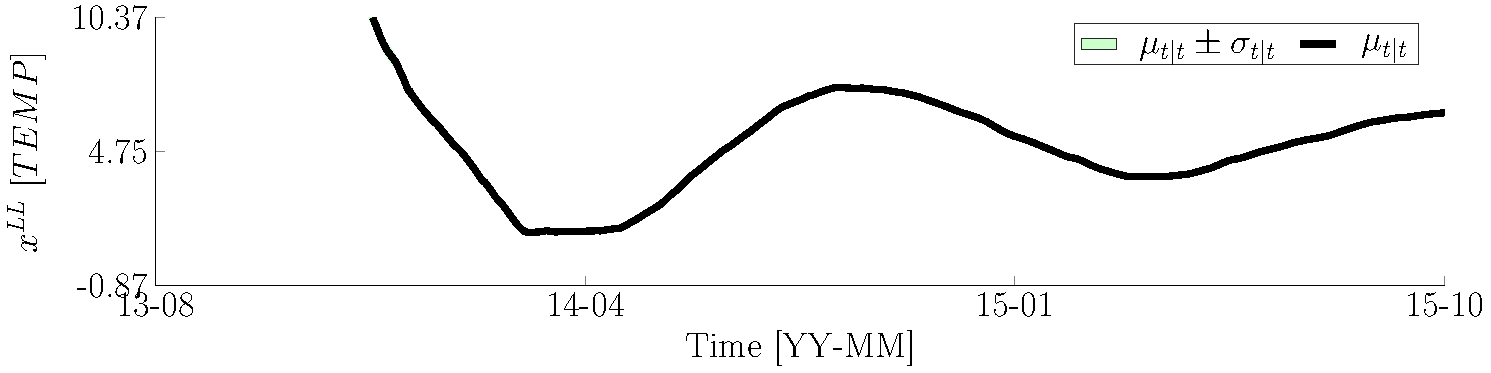
\includegraphics[width=0.9\linewidth]{./docfigs/Example_DISPTEMPSIM/default/TEMP_LL_1.pdf} 
%\caption{Estimated temperature local level component.}
%\end{subfigure}
%\begin{subfigure}{\linewidth}
%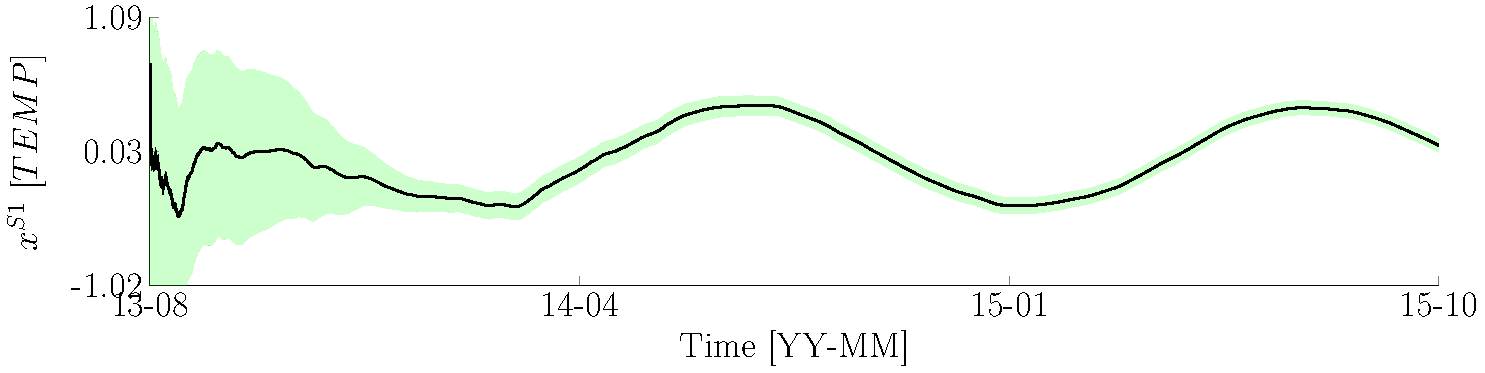
\includegraphics[width=0.9\linewidth]{./docfigs/Example_DISPTEMPSIM/default/TEMP_S1_2.pdf} 
%\caption{Estimated temperature yearly component (first hidden state)}
%\end{subfigure}
%\begin{subfigure}{\linewidth}
%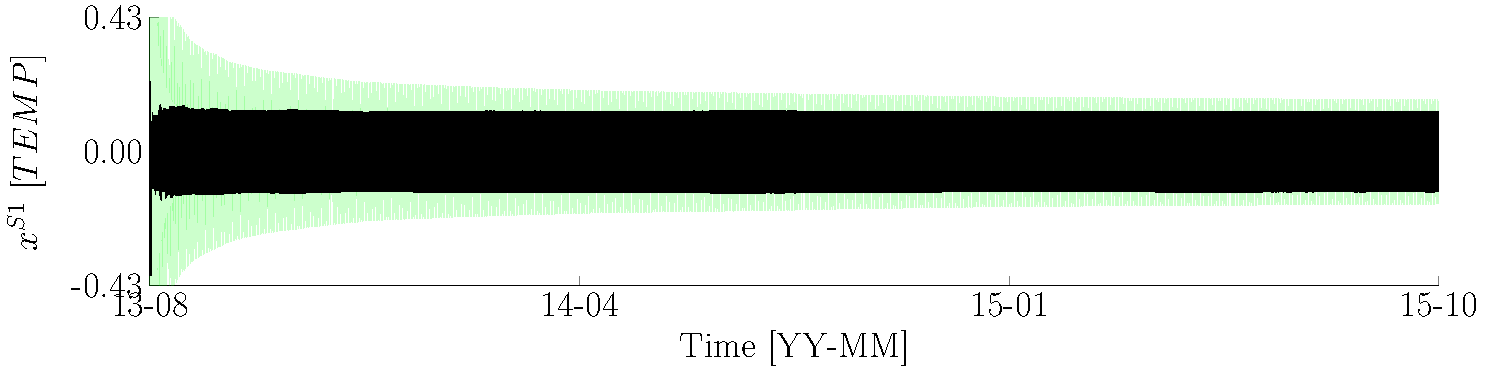
\includegraphics[width=0.9\linewidth]{./docfigs/Example_DISPTEMPSIM/default/TEMP_S1_4.pdf} 
%\caption{Estimated temperature daily component (first hidden state)}
%\end{subfigure}
%\begin{subfigure}{\linewidth}
%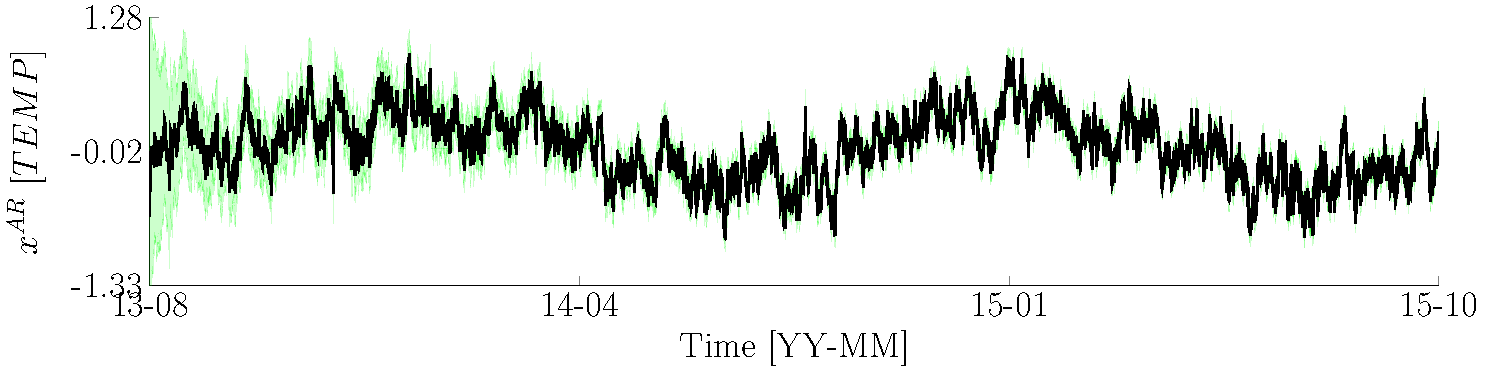
\includegraphics[width=0.9\linewidth]{./docfigs/Example_DISPTEMPSIM/default/TEMP_AR_6.pdf} 
%\caption{Estimated temperature autoregressive component}
%\end{subfigure}
%\caption{Estimated results using OpenBDLM default model parameters and default initial hidden states. The hidden states are estimated from the data presented in Figure~\ref{fig:DataSummaryDefaultPreProcessed2}a. The solid line and shaded area represent the mean and standard deviation of the estimated hidden states, respectively.}
%\label{fig:DISPTEMPSIMDefaultDefaultExample2}
%\end{figure*}

%\begin{figure*}[h!]
%\centering
%\begin{subfigure}{\linewidth}
%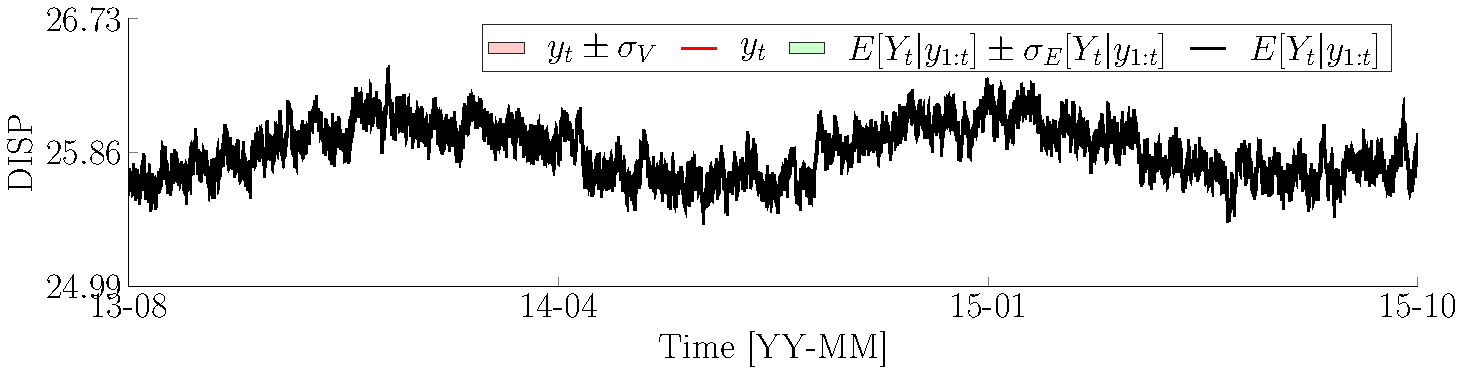
\includegraphics[width=0.9\linewidth]{./docfigs/Example_DISPTEMPSIM/optim_param_default_initialhiddenstate/DISP_ObservedPredicted.pdf}
%\caption{Observed and estimated displacement data} 
%\end{subfigure}
%\begin{subfigure}{\linewidth}
%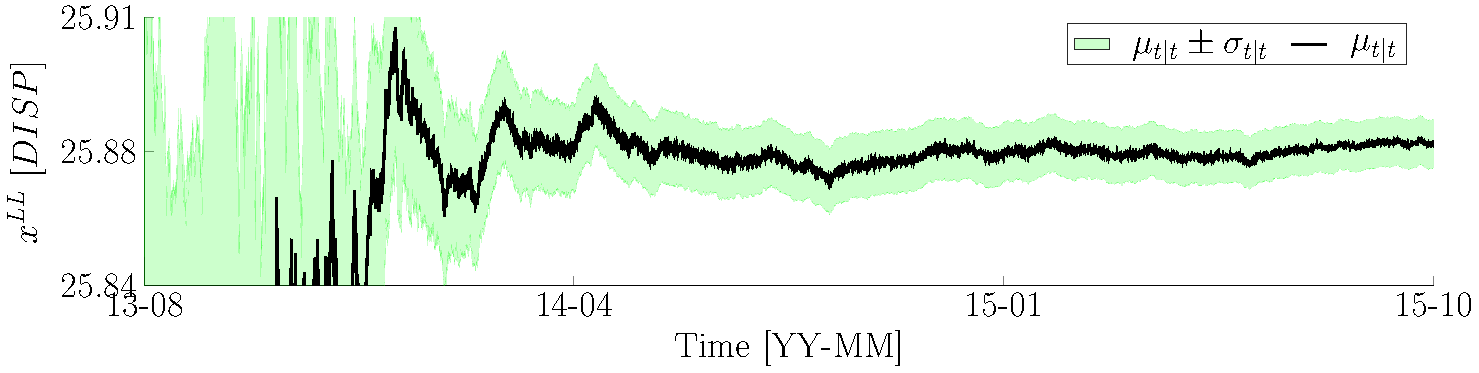
\includegraphics[width=0.9\linewidth]{./docfigs/Example_DISPTEMPSIM/optim_param_default_initialhiddenstate/DISP_LL_1.pdf}
%\caption{Estimated displacement local level component.}
%\end{subfigure}
%\begin{subfigure}{\linewidth}
%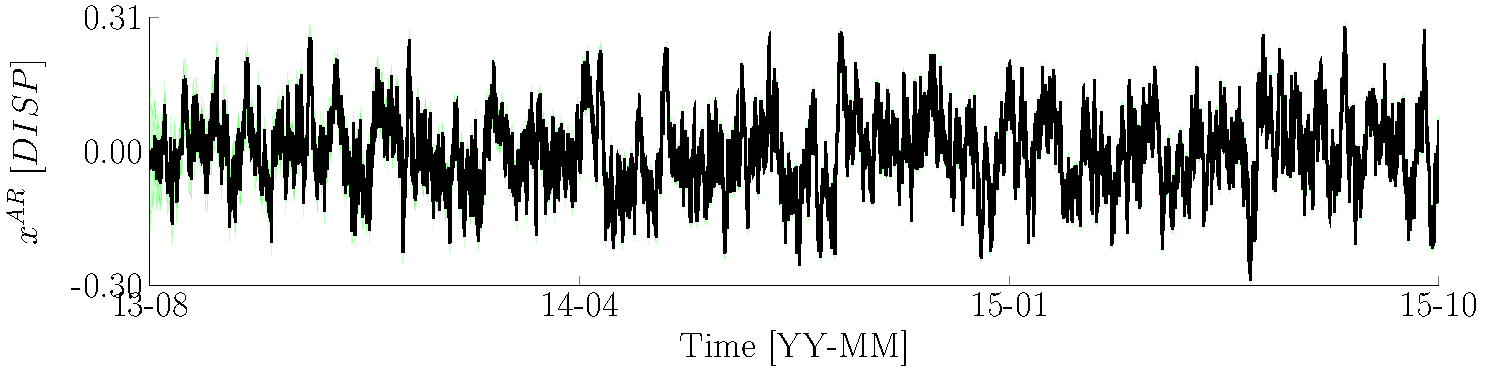
\includegraphics[width=0.9\linewidth]{./docfigs/Example_DISPTEMPSIM/optim_param_default_initialhiddenstate/DISP_AR_2.pdf}
%\caption{Estimated displacement autoregressive component.}
%\end{subfigure}
%\end{figure*}
%\begin{figure*}[h!]
%\ContinuedFloat
%\begin{subfigure}{\linewidth}
%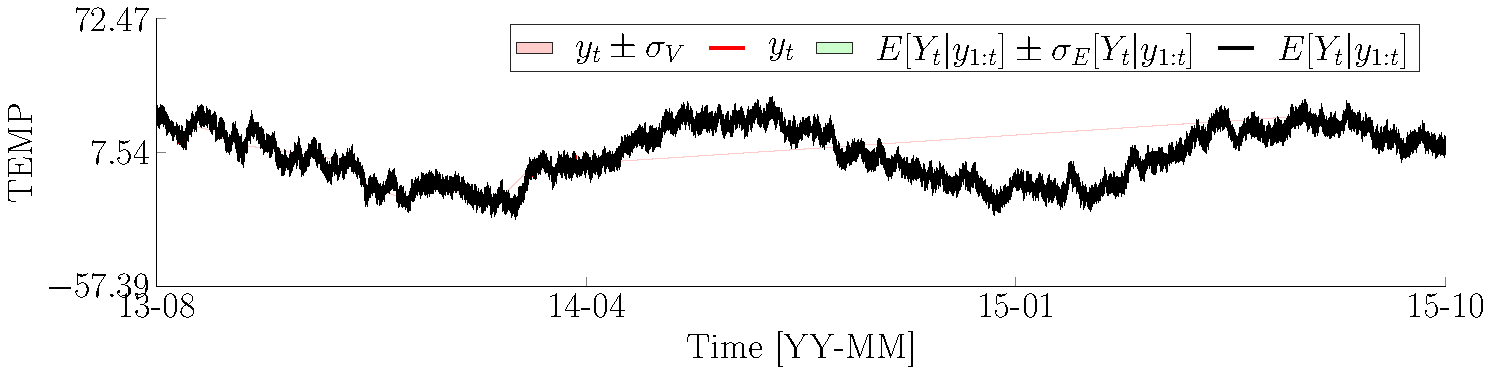
\includegraphics[width=0.9\linewidth]{./docfigs/Example_DISPTEMPSIM/optim_param_default_initialhiddenstate/TEMP_ObservedPredicted.pdf} 
%\caption{Observed and estimated temperature data}
%\end{subfigure}
%\begin{subfigure}{\linewidth}
%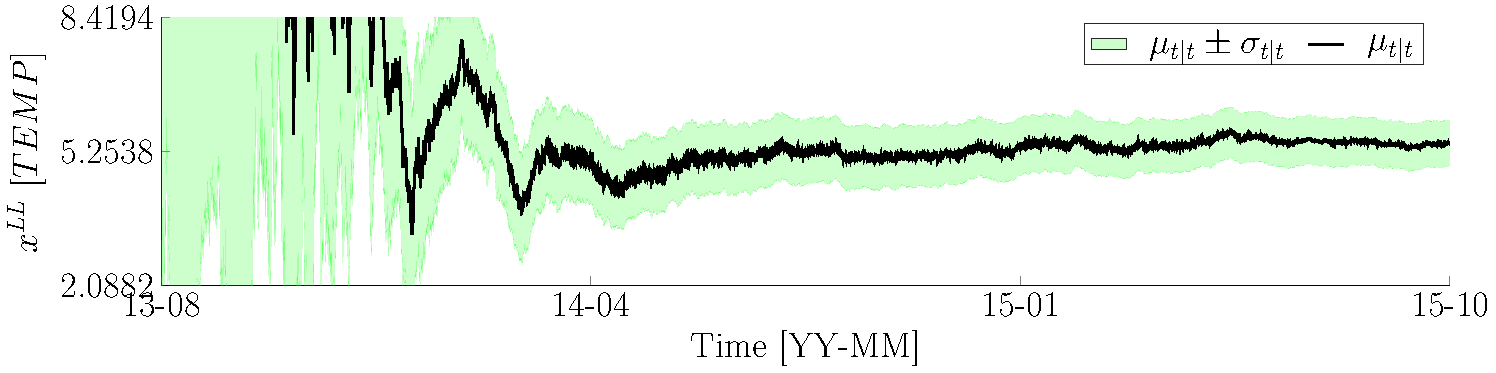
\includegraphics[width=0.9\linewidth]{./docfigs/Example_DISPTEMPSIM/optim_param_default_initialhiddenstate/TEMP_LL_1.pdf} 
%\caption{Estimated temperature local level component.}
%\end{subfigure}
%\begin{subfigure}{\linewidth}
%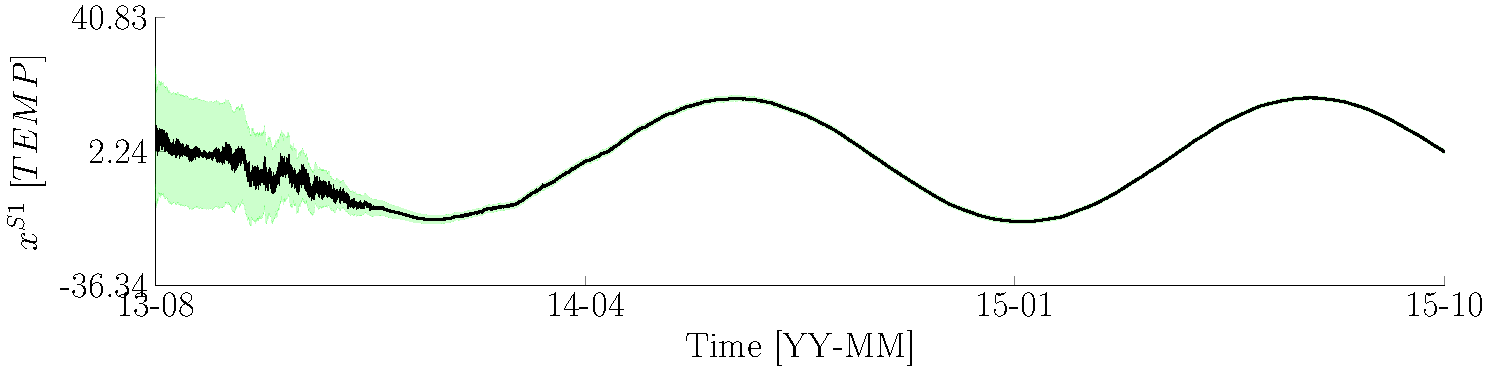
\includegraphics[width=0.9\linewidth]{./docfigs/Example_DISPTEMPSIM/optim_param_default_initialhiddenstate/TEMP_S1_2.pdf} 
%\caption{Estimated temperature yearly component (first hidden state)}
%\end{subfigure}
%\begin{subfigure}{\linewidth}
%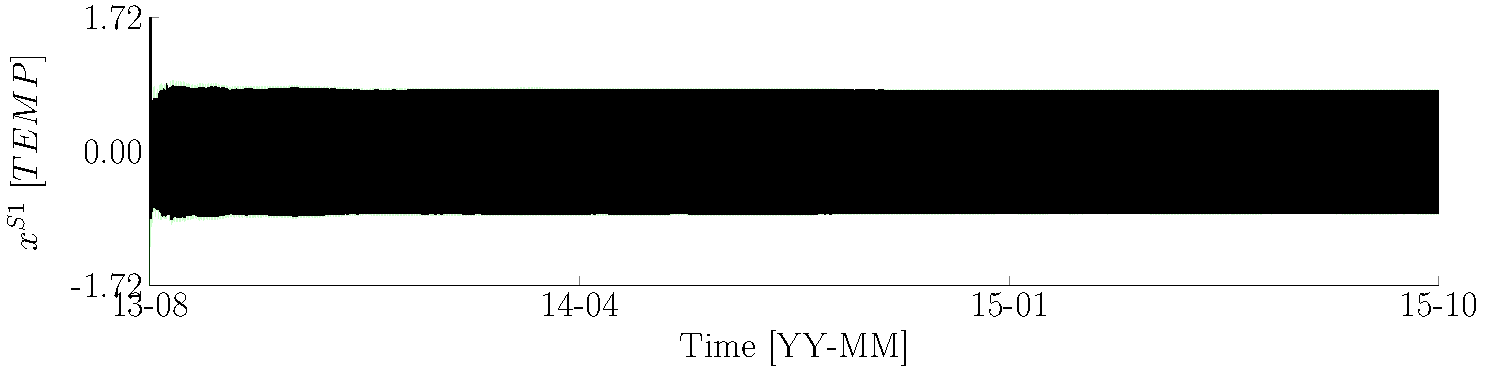
\includegraphics[width=0.9\linewidth]{./docfigs/Example_DISPTEMPSIM/optim_param_default_initialhiddenstate/TEMP_S1_4.pdf} 
%\caption{Estimated temperature daily component (first hidden state)}
%\end{subfigure}
%\begin{subfigure}{\linewidth}
%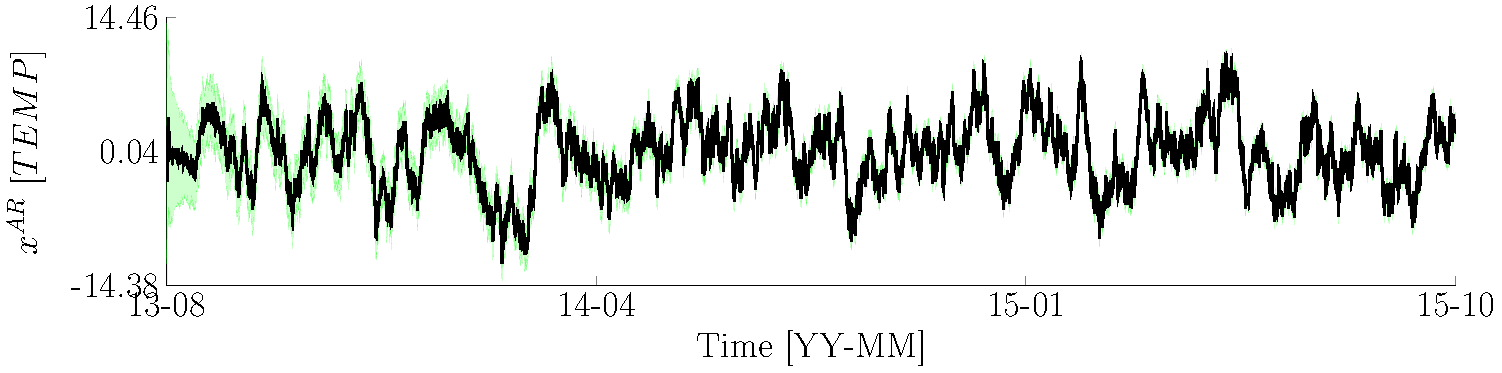
\includegraphics[width=0.9\linewidth]{./docfigs/Example_DISPTEMPSIM/optim_param_default_initialhiddenstate/TEMP_AR_6.pdf} 
%\caption{Estimated temperature autoregressive component}
%\end{subfigure}
%\caption{Estimated results using OpenBDLM optimized model parameters and default initial hidden states. The hidden states are estimated from the data presented in Figure~\ref{fig:DataSummaryDefaultPreProcessed2}a. The solid line and shaded area represent the mean and standard deviation of the estimated hidden states, respectively.}
%\label{fig:DISPTEMPSIMOptimizedDefaultExample2}
%\end{figure*}

\begin{figure*}[h!]
\centering
\begin{subfigure}{\linewidth}
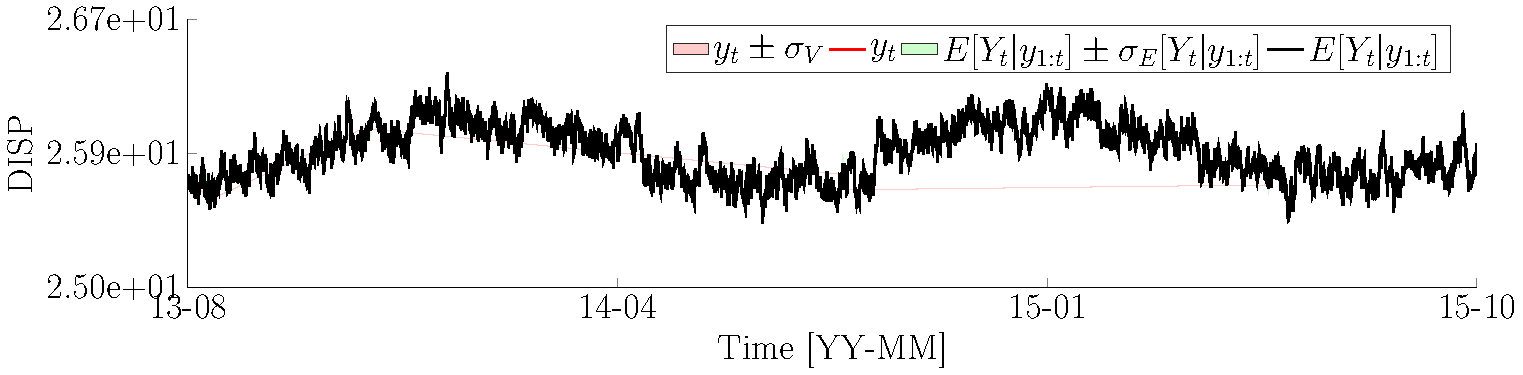
\includegraphics[width=0.9\linewidth]{./docfigs/Example_DISPTEMPSIM/optim_param_optim_initialhiddenstate/DISP_ObservedPredicted.pdf}
\caption{Observed and estimated displacement data} 
\end{subfigure}
\begin{subfigure}{\linewidth}
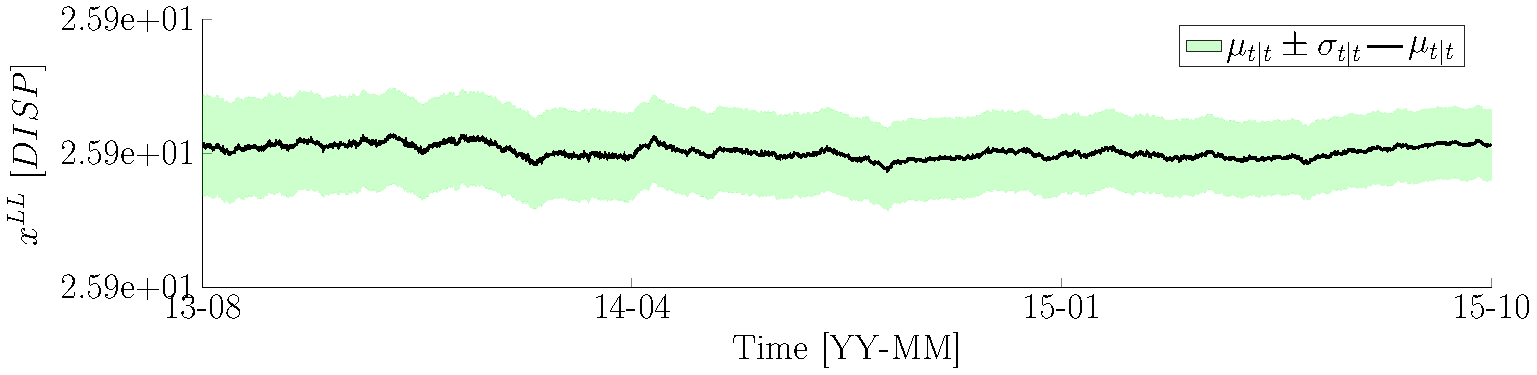
\includegraphics[width=0.9\linewidth]{./docfigs/Example_DISPTEMPSIM/optim_param_optim_initialhiddenstate/DISP_LL_1.pdf}
\caption{Estimated displacement local level component.}
\end{subfigure}
\begin{subfigure}{\linewidth}
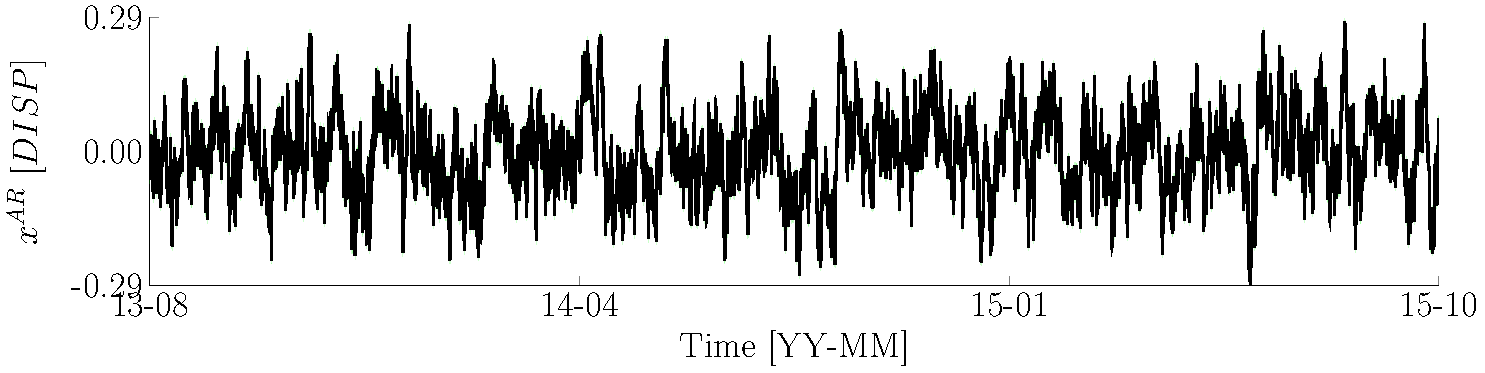
\includegraphics[width=0.9\linewidth]{./docfigs/Example_DISPTEMPSIM/optim_param_optim_initialhiddenstate/DISP_AR_2.pdf}
\caption{Estimated displacement autoregressive component.}
\end{subfigure}
\end{figure*}
\begin{figure*}[h!]
\ContinuedFloat
\begin{subfigure}{\linewidth}
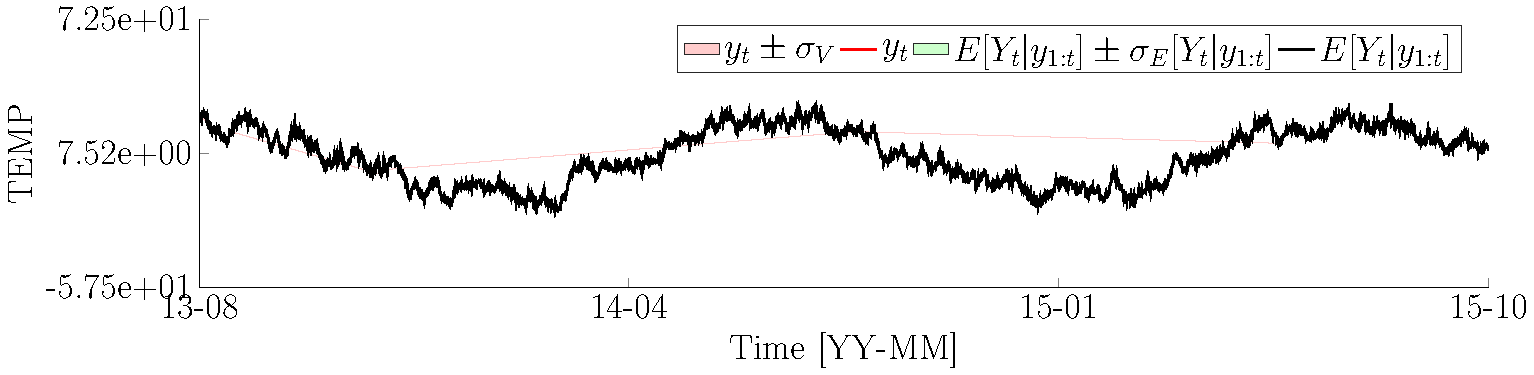
\includegraphics[width=0.9\linewidth]{./docfigs/Example_DISPTEMPSIM/optim_param_optim_initialhiddenstate/TEMP_ObservedPredicted.pdf} 
\caption{Observed and estimated temperature data}
\end{subfigure}
\begin{subfigure}{\linewidth}
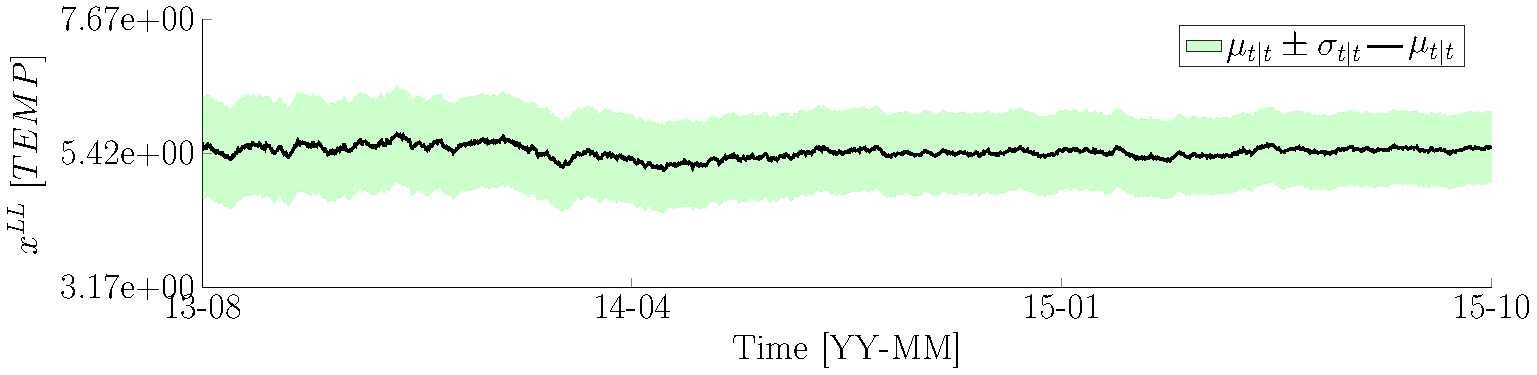
\includegraphics[width=0.9\linewidth]{./docfigs/Example_DISPTEMPSIM/optim_param_optim_initialhiddenstate/TEMP_LL_1.pdf} 
\caption{Estimated temperature local level component.}
\end{subfigure}
\begin{subfigure}{\linewidth}
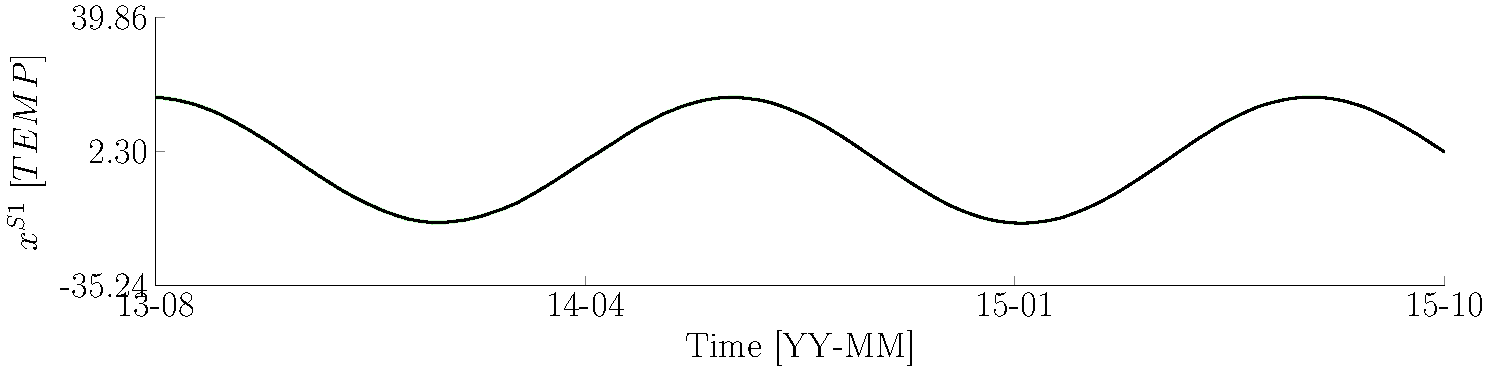
\includegraphics[width=0.9\linewidth]{./docfigs/Example_DISPTEMPSIM/optim_param_optim_initialhiddenstate/TEMP_S1_2.pdf} 
\caption{Estimated temperature yearly component (first hidden state)}
\end{subfigure}
\begin{subfigure}{\linewidth}
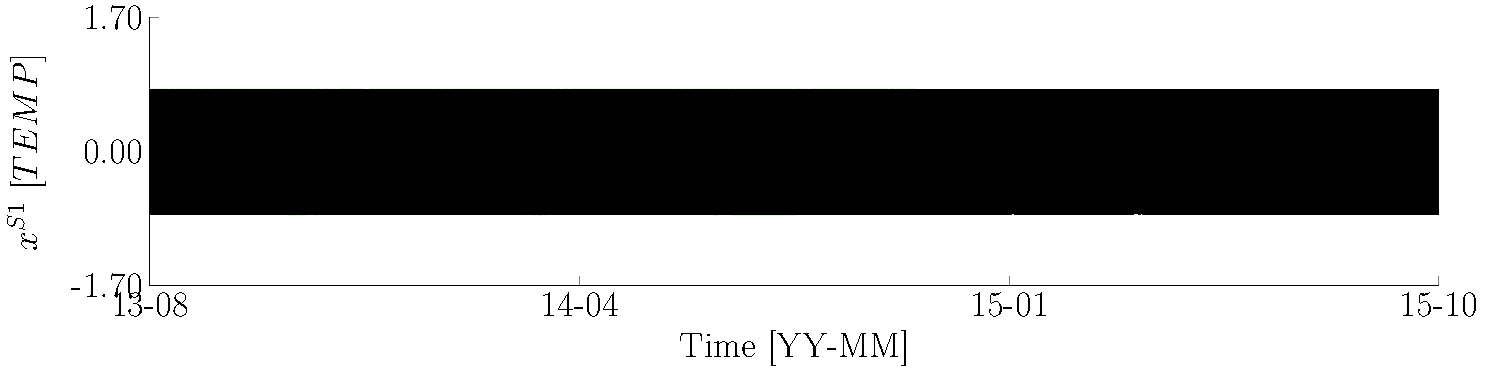
\includegraphics[width=0.9\linewidth]{./docfigs/Example_DISPTEMPSIM/optim_param_optim_initialhiddenstate/TEMP_S1_4.pdf} 
\caption{Estimated temperature daily component (first hidden state)}
\end{subfigure}
\begin{subfigure}{\linewidth}
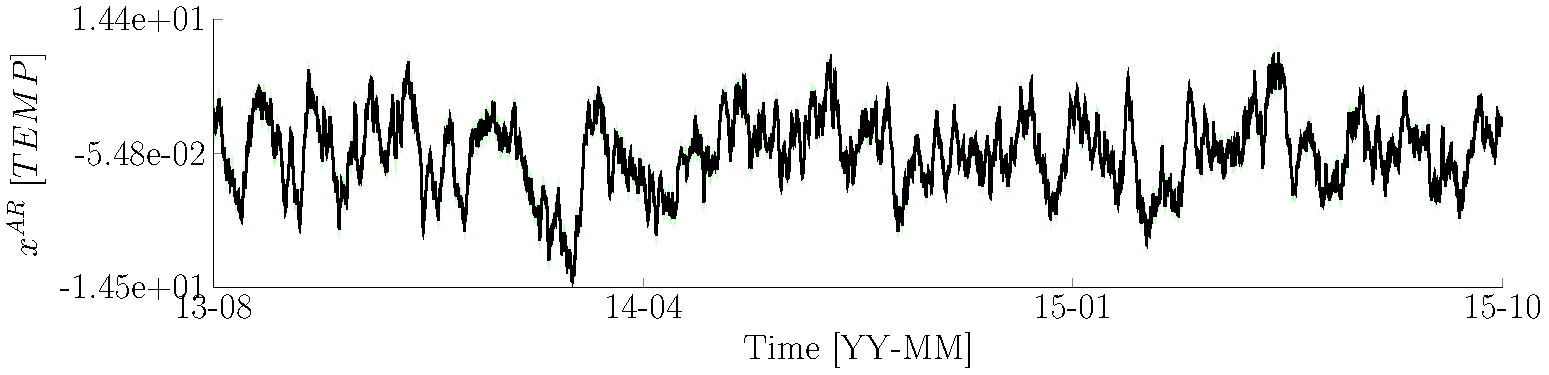
\includegraphics[width=0.9\linewidth]{./docfigs/Example_DISPTEMPSIM/optim_param_optim_initialhiddenstate/TEMP_AR_6.pdf} 
\caption{Estimated temperature autoregressive component}
\end{subfigure}
\caption{Estimated results using OpenBDLM optimized model parameters and optimized initial hidden states. The hidden states are estimated from the data presented in Figure~\ref{fig:DataSummaryDefaultPreProcessed2}a. The solid line and shaded area represent the mean and standard deviation of the estimated hidden states, respectively.}
\label{fig:DISPTEMPSIMOptimizedOptimizedExample2}
\end{figure*}